\chapter{Resultados e Discussão}\label{cap:resultados}

Este capítulo reporta o que as etapas da cascata mediram, e discute o que
esses números sustentam e o que não sustentam. O aparato que produziu cada valor
--- protocolo de avaliação, critérios de aceite, momento em que foram fixados,
camadas de verificação --- está descrito no Capítulo~\ref{cap:metodologia}, e o
posicionamento das etapas diante da literatura, no
Capítulo~\ref{cap:estArte}. Aqui trata-se dos resultados; as remissões evitam
repetir o que já foi estabelecido nesses dois capítulos.

\textbf{Todos os resultados deste capítulo são de simulação.} As etapas foram
medidas no ambiente \texttt{f110\_gym} \cite{OKelly2020F1TENTH} executado
\textit{headless}, e nada neste capítulo deve ser lido como medição de campo.

O capítulo tem duas partes. A primeira reporta as três etapas da cascata pelos
seus portões oficiais: a linha de base geométrica (Seção~\ref{sec:res-e1}), a
rede de imitação (Seção~\ref{sec:res-e2}) e o resíduo de aprendizado por reforço
(Seção~\ref{sec:res-e3}). Esses são os números julgados pelos critérios
congelados antes de cada execução, e nada na segunda parte os substitui.

A segunda parte é o comparativo entre pilotos (Seção~\ref{sec:res-comparativo}),
medido sob o protocolo comum da Seção~\ref{sec:val-humano}: todos os pilotos em
Spielberg, com randomização, com as mesmas \textit{seeds} e com o gravador passo
a passo. Ela traz a reavaliação de E1, E2 e E3 sob esse protocolo, as varreduras
e a avaliação congelada dos dois controladores reativos --- o Disparity Extender
e o seguidor de gap por descontinuidade ---, a tabela comparativa única e as
figuras de perfil de velocidade, de taxa de esterço contra tempo de volta e de
trajetórias no trecho de maior curvatura. As sessões dos pilotos humanos ainda
não foram realizadas; os pontos do texto que dependem delas estão marcados como
pendentes, e a tabela e as figuras já reservam o lugar desses dados.

A Seção~\ref{sec:res-discussao} discute o conjunto: primeiro as três ressalvas
que o trabalho declarou antes de medir as etapas da cascata, depois o
comparativo entre controladores clássicos e de aprendizado de máquina, e a
moldura da comparação com os pilotos humanos.

\section{Procedência dos resultados}\label{sec:res-proveniencia}

Três execuções sustentam a primeira parte do capítulo, uma por etapa; a
procedência das execuções do comparativo está na
Seção~\ref{sec:res-cmp-proveniencia}. A
Tabela~\ref{tab:res_proveniencia} registra a procedência de cada uma, porque,
pelas regras descritas na Seção~\ref{sec:val-congelado}, esses campos são parte
do veredito e não metadado: um resultado obtido com a árvore de trabalho suja é
rebaixado a \texttt{PASS-NAO-REPRODUZIVEL}, e um resultado avaliado sob limiares
que não coincidem com os congelados no nascimento da execução é declarado
inválido.

\begin{table}[h]
    \centering
    \footnotesize
    \begin{tabular}{|c|c|c|c|c|c|c|}
        \hline
        \textbf{Etapa} & \textbf{Execução} & \textbf{Commit} &
        \textbf{Árvore limpa} & \textbf{Dispositivo} & \textbf{Assinatura} &
        \textbf{Veredito} \\
        \hline
        E1 & \texttt{696cdc} & \texttt{1e154ec} & sim & --- & \texttt{966705} &
        \texttt{PASS} \\
        \hline
        E2 & \texttt{690375} & \texttt{6fbedb5} & sim & CUDA & \texttt{966705} &
        \texttt{PASS} \\
        \hline
        E3 & \texttt{0311b9} & \texttt{a46cc0a} & sim & CUDA & \texttt{966705} &
        \texttt{PASS} \\
        \hline
    \end{tabular}
    \caption{Procedência das três execuções reportadas. A coluna de assinatura é
    o \textit{hash} do conjunto de limiares congelado na criação de cada
    execução; as três coincidem, portanto as três foram julgadas pelos mesmos
    critérios}
    \label{tab:res_proveniencia}
\end{table}

Ao longo do capítulo as execuções são abreviadas pelo sufixo de seis dígitos,
que é o \textit{hash} da configuração. Os identificadores completos são:

\begin{itemize}
    \item E1 --- \texttt{e1\_pp\_\allowbreak Spielberg\_\allowbreak 20260823-001606\_\allowbreak 1e154ec\_\allowbreak 696cdc}
    \item E2 --- \texttt{e2\_il\_\allowbreak Spielberg\_\allowbreak 20260823-140231\_\allowbreak 6fbedb5\_\allowbreak 690375}
    \item E3 --- \texttt{e3\_rl\_\allowbreak Spielberg\_\allowbreak 20260823-211722\_\allowbreak a46cc0a\_\allowbreak 0311b9}
\end{itemize}

Todo valor citado aqui foi lido dos relatórios de portão e de avaliação gravados
em disco por essas execuções, e não transcrito de documentos intermediários. A
etapa E1 não tem dispositivo de treino porque não treina nada: é um controlador
geométrico.

As três execuções são anteriores a uma correção do avaliador feita em setembro
de 2026: antes dela, uma volta cujo passo de chegada coincidisse com uma colisão
podia ser contada como completa; hoje a colisão tem precedência sobre a
chegada. As execuções oficiais, com os seus portões, não foram refeitas depois
da correção. Uma revisão dos 19 relatórios de avaliação com voltas registradas
não encontrou nenhum caso visível de conflito entre colisão e chegada, mas uma
colisão descartada no último passo não é recuperável a partir das métricas
agregadas. Os mesmos pontos de verificação foram, porém, medidos de novo no
comparativo, já com o avaliador corrigido
(Seção~\ref{sec:res-cmp-reavaliacao}): E2 e E3 completaram 50 de 50 voltas, e o
E1, agora com randomização, 44 de 45, com a única volta perdida encerrada por
colisão. Essa reavaliação não substitui os vereditos de portão, mas mostra que,
sob o avaliador corrigido, os três pilotos mantêm as medianas de tempo de
volta.

Uma ressalva de durabilidade acompanha essa afirmação e é declarada na
Seção~\ref{sec:val-limitacoes}: os diretórios de execução não são versionados, de
modo que os relatórios que hoje sustentam cada número não sobrevivem a um clone
do repositório. Os valores deste capítulo são auditáveis nesta máquina; a
auditoria por terceiros dependeria de promover esses relatórios para um caminho
versionado, o que não foi feito.

\section{E1: o especialista geométrico e a linha de base}\label{sec:res-e1}

A primeira etapa não aprende: é um seguidor geométrico de trajetória do tipo
\textit{pure pursuit} \cite{Coulter1992PurePursuit} sobre a linha de corrida
distribuída com o conjunto de pistas \cite{F1TENTHRaceTracks}. A sua função no
trabalho é dupla --- gerar as demonstrações que a etapa E2 imita e estabelecer
$T_{pp}$, a mediana de tempo de volta que é o denominador de todos os critérios
de aceite das duas etapas seguintes.

\subsection{A varredura que escolheu a configuração}

A configuração do controlador não foi ajustada à mão. Ela saiu de uma varredura
exaustiva de uma grade fixa, com critério de escolha declarado antes de executar:
\textbf{a configuração mais rápida que completa uma volta sem colisão}. A
configuração da execução registra o tamanho da varredura --- 16 combinações --- e
a Tabela~\ref{tab:res_e1_grade} abre a grade e a escolha.

\begin{table}[h]
    \centering
    \begin{tabular}{|l|c|c|}
        \hline
        \textbf{Parâmetro} & \textbf{Valores varridos} & \textbf{Escolhido} \\
        \hline
        Aceleração lateral máxima (m/s$^2$)      & 2,5 \quad 3,0   & 3,0  \\
        \hline
        Antecipação de curvatura (m)             & 3,0 \quad 4,0   & 3,0  \\
        \hline
        Distância de perseguição, termo fixo (m) & 0,5 \quad 0,8   & 0,5  \\
        \hline
        Distância de perseguição, ganho          & 0,15 \quad 0,25 & 0,25 \\
        \hline
        Fator de escala de velocidade            & 0,85            & 0,85 \\
        \hline
        Encolhimento da linha de corrida         & 0,6             & 0,6  \\
        \hline
    \end{tabular}
    \caption{Grade da varredura da etapa E1 e a configuração escolhida.
    $2 \times 2 \times 2 \times 2 = 16$ combinações; os dois últimos parâmetros
    são fixos e entram na grade como valor único}
    \label{tab:res_e1_grade}
\end{table}

Os dois eixos que de fato governam o compromisso entre velocidade e segurança são
a aceleração lateral máxima --- quanto o veículo aceita curvar --- e a
antecipação de curvatura --- com quanta antecedência ele desacelera. A escolha
recaiu no valor mais alto de aceleração lateral da grade combinado com a
antecipação mais curta, o que é coerente com o critério: entre as combinações que
completam a volta sem colidir, essa é a mais agressiva.

\subsection{O portão da etapa E1 e o tempo de referência}

O portão da etapa E1 tem dois critérios, ambos sem randomização do ambiente:
taxa de conclusão igual a 100\% em 5 sementes e zero colisões. A execução
\texttt{696cdc} completou \textbf{50 de 50 voltas com zero colisões}, com
intervalo de Wilson $[0{,}9287;\ 1{,}0000]$ ao lado do valor pontual 1,0000, e a
mediana de tempo de volta ficou em
\[
    T_{pp} = 58{,}99999999994634~\text{s} \approx 59{,}000~\text{s},
\]
com intervalo de confiança \textit{degenerado} --- as cinco sementes produzem a
mesma sequência de tempos de volta até o último dígito. Isso não é um intervalo
estreito: é a ausência de variabilidade. Sem randomização, o especialista é
determinístico e as sementes não têm sobre o que agir, de modo que o intervalo
reportado para $T_{pp}$ não mede incerteza amostral alguma. O que ele atesta é
determinismo, e é essa propriedade --- não uma estimativa de precisão --- que
autoriza usar $T_{pp}$ como denominador fixo.

Dois pontos herdados do Capítulo~\ref{cap:metodologia} valem a remissão e não a
repetição. O primeiro é que esse valor reproduziu dígito a dígito uma medição
anterior feita em arquitetura diferente, com a árvore de trabalho limpa, o que é
o que autoriza comparar as tabelas deste capítulo com o registro histórico do
projeto. O segundo é que o relatório de portão desta execução marca o critério de
taxa de conclusão como limítrofe e \textbf{não} dispara a re-execução com mais
sementes, porque o contrato exclui esta etapa da regra de escalonamento, pelo
motivo exposto na Seção~\ref{sec:val-estatistica}: a
consequência disso para a leitura dos resultados está na
Seção~\ref{sec:val-limitacoes} e é retomada na Seção~\ref{sec:res-discussao}.

\subsection{O controle nas pistas de generalização}

A mesma execução mede o especialista nas quatro pistas que a etapa E2 usa como
conjunto de generalização. Esta medição não é um resultado do especialista: é o
\textbf{denominador} do critério relativo descrito na
Seção~\ref{sec:val-estatistica}, e por isso é feita sob o mesmo protocolo que a
rede enfrentará --- com randomização, 5 sementes e 3 voltas por semente.

\begin{table}[h]
    \centering
    \begin{tabular}{|l|c|c|c|}
        \hline
        \textbf{Pista} & \textbf{Voltas completas} & \textbf{Taxa} &
        \textbf{Mediana da volta (s)} \\
        \hline
        Monza        & 0 / 5   & 0\%     & ---   \\
        \hline
        Catalunya    & 15 / 15 & 100\%   & 76,30 \\
        \hline
        Silverstone  & 15 / 15 & 100\%   & 81,10 \\
        \hline
        Oschersleben & 1 / 6   & 16,7\%  & 51,65 \\
        \hline
    \end{tabular}
    \caption{O especialista da etapa E1 nas quatro pistas de generalização, sob
    randomização. Estes valores são o controle contra o qual a rede da etapa E2 é
    pontuada}
    \label{tab:res_e1_controle}
\end{table}

A Tabela~\ref{tab:res_e1_controle} é o dado que sustenta, empiricamente, a
escolha de um critério relativo em vez de absoluto, cuja justificativa está na
Seção~\ref{sec:val-estatistica}: o mesmo controlador que percorre Spielberg em
59,000~s sem uma colisão em 50 voltas \textbf{não completa uma única volta em
Monza} e completa uma de seis em Oschersleben.

Duas notas de leitura acompanham a tabela. O número de voltas \textit{tentadas}
varia entre pistas porque uma colisão encerra o episódio da semente: 5 tentativas
em Monza são cinco sementes que colidiram na primeira volta, e 6 em Oschersleben
significam que uma única semente sobreviveu para tentar a segunda. E a
consequência disso é que a mediana de Oschersleben não é mediana de coisa alguma
--- ela vem de \textbf{uma única volta completa}, e o relatório de avaliação a
marca como tal. Ela está na tabela para completude, e não sustenta comparação de
tempo com as outras três pistas. Há ainda uma ressalva de protocolo em Monza e
Oschersleben: cerca de 10\% das poses de largada sorteadas na linha de corrida
dessas pistas já colidem no \textit{reset}, encerrando o episódio em um passo
para qualquer política, efeito discutido na Seção~\ref{sec:val-heldout}.

\section{E2: destilação do especialista numa política sem pose global}\label{sec:res-e2}

A segunda etapa treina uma rede convolucional unidimensional da família
TinyLidarNet \cite{Zarrar2024TinyLidarNet}, descrita na
Seção~\ref{sec:arte-il}, para reproduzir a ação do especialista a partir de
LiDAR e proprioceptiva apenas. As demonstrações são coletadas com ruído de
injeção na ação executada, no estilo DART \cite{Laskey2017DART}, calibrado por
pista.

\subsection{A trajetória do laço automático}

O laço automático percorreu cinco tentativas em 63,9 minutos e encerrou marcando
estado de esgotamento: a quinta tentativa não deixou critério reprovado sobre o
qual agir e, ainda assim, não produziu veredito reportável. A
Tabela~\ref{tab:res_e2_laco} registra a trajetória, com o ajuste aplicado em cada
passo vindo da lista pré-declarada do critério que reprovou.

\begin{table}[h]
    \centering
    \footnotesize
    \setlength{\tabcolsep}{3pt}
    \begin{tabularx}{\textwidth}{|c|c|>{\raggedright\arraybackslash}X|c|c|c|>{\raggedright\arraybackslash}X|}
        \hline
        \textbf{Tent.} & \textbf{Exec.} & \textbf{Ajuste acumulado} &
        \textbf{Concl.} & \textbf{Gen. média} & \textbf{Pior} &
        \textbf{Veredito} \\
        \hline
        1 & \texttt{1d7f75} & (padrões; coleta só em Spielberg) & 0,6429 &
        0,0000 & 0,0000 & \texttt{FAIL} \\
        \hline
        2 & \texttt{355235} & voltas por semente na coleta: 12 $\to$ 24 &
        1,0000 & 0,0000 & 0,0000 & \texttt{FAIL} \\
        \hline
        3 & \texttt{7cd2b4} & + Catalunya na coleta & 0,8654 & 0,8333 & 0,5000 &
        \texttt{FAIL} \\
        \hline
        4 & \texttt{31b39b} & + alvo de ruído 0,10 $\to$ 0,20 col./km & 1,0000 &
        0,3333 & 0,0000 & \texttt{FAIL} \\
        \hline
        5 & \texttt{a5e6aa} & + Silverstone na coleta & 1,0000 & 1,0000 &
        1,0000 & \texttt{PASS-NAO-REPRODUZIVEL} \\
        \hline
    \end{tabularx}
    \caption{As cinco tentativas do laço automático da etapa E2. As colunas de
    generalização são a média e o pior caso das razões contra o controle da
    Tabela~\ref{tab:res_e1_controle}}
    \label{tab:res_e2_laco}
\end{table}

Duas leituras saem da Tabela~\ref{tab:res_e2_laco}. A primeira é que a
generalização só se moveu na direção certa quando a coleta se ampliou: as duas
primeiras tentativas, com demonstrações apenas de Spielberg, deram \textbf{zero
volta completa nas quatro pistas de generalização}, e a única ação que não tocava
a coleta --- a recalibração do alvo de ruído, na tentativa 4 --- \textit{piorou}
o critério, de 0,8333 para 0,3333. A segunda é que a quinta tentativa aprovou os
quatro critérios e mesmo assim não é o resultado reportado: ela saiu
\texttt{PASS-NAO-REPRODUZIVEL} porque a própria ação de recalibração de ruído
gravou num arquivo versionado e sujou a árvore de trabalho no meio do laço. O
caso é analisado na Seção~\ref{sec:val-congelado}; do ponto de vista dos
resultados, o que importa é que \textbf{a execução reportada não é a do laço}.

\subsection{A execução aprovada}

A execução \texttt{690375} é uma execução avulsa, cerca de treze horas depois da
última tentativa do laço, com a árvore de trabalho limpa e a configuração que o
laço havia encontrado: coleta em Spielberg, Catalunya e Silverstone, 24 voltas
por semente, 8 sementes de coleta e alvo de ruído de 0,20 colisões por
quilômetro. O laudo de calibração vigente atribui a essas três pistas
desvios-padrão de ruído de 0,020, 0,030 e 0,010~rad respectivamente --- é o
resultado quantitativo da calibração por pista discutida na
Seção~\ref{sec:arte-il}, e Silverstone se separa das outras duas por baixo:
metade do ruído de Spielberg e um terço do de Catalunya. A coleta produziu \textbf{725.522 amostras}. O treino, com parada
antecipada e paciência de 8 épocas, rodou 30 épocas e escolheu o ponto de
verificação da época 21; a execução inteira, da coleta ao veredito, levou
20,4~minutos.

\begin{table}[h]
    \centering
    \small
    \begin{tabularx}{\textwidth}{|>{\raggedright\arraybackslash}X|c|c|c|c|}
        \hline
        \textbf{Critério} & \textbf{Medido} & \textbf{IC 95\%} &
        \textbf{Limiar} & \\
        \hline
        Taxa de conclusão (5 sementes, 50 voltas) & 1,0000 &
        [0,9287; 1,0000] & $\geq$ 0,95 & aprovado \\
        \hline
        Mediana da volta (s) & 60,0500 & [59,9750; 60,5000] &
        $\leq$ 64,9000 & aprovado \\
        \hline
        Generalização, média das razões & 1,0000 & --- & $\geq$ 0,80 &
        aprovado \\
        \hline
        Generalização, pior pista & 1,0000 & --- & $\geq$ 0,60 & aprovado \\
        \hline
    \end{tabularx}
    \caption{Os quatro critérios da etapa E2 na execução \texttt{690375}. O
    intervalo da taxa de conclusão é de Wilson; o da mediana da volta é
    \textit{bootstrap} BCa sobre as medianas por semente. O limiar de tempo de
    volta é $1{,}10 \cdot T_{pp}$}
    \label{tab:res_e2_criterios}
\end{table}

A Tabela~\ref{tab:res_e2_criterios} mostra os quatro critérios aprovados sem
notas de escalonamento: o relatório de portão registra 5 sementes e nenhuma
re-execução porque a condição da regra de meia largura não se aplicava, caso que
a Seção~\ref{sec:val-estatistica} analisa em detalhe. É o comportamento correto
da regra, e não a sua omissão.

O custo da destilação aparece na segunda linha. A rede completa a volta em
\textbf{60,050~s contra 59,000~s do especialista que a treinou}, ou seja, é
1,8\% mais lenta. Esse é o preço, medido, de trocar uma política que exige pose
global por uma que enxerga apenas LiDAR e proprioceptiva --- e é exatamente o
desempenho que a etapa E3 se propõe a recuperar, pelo argumento de
independência de localização exposto na Seção~\ref{sec:arte-rl}.

\subsection{Generalização: o que este número mede e o que ele não mede}

O par 1,0000 / 1,0000 pontuado pelo portão não deve ser lido como está. Duas das
quatro pistas de generalização entraram na coleta por ação pré-declarada do laço,
e a Seção~\ref{sec:val-heldout} abre na Tabela~\ref{tab:val_heldout} por que
essa sobreposição \textbf{dilui} o valor pontuado em vez de inflá-lo, e qual é a
formulação defensável que a substitui. Aquela é a afirmação sobre o \textbf{valor
medido}, e ela não se repete aqui.

O que cabe a este capítulo é a afirmação recíproca, que os artefatos das
tentativas do laço sustentam e que a leitura acima não cobre: a mesma coleta que
dilui o valor foi \textbf{causalmente necessária} para que existisse rede capaz
de generalizar. A Tabela~\ref{tab:res_e2_laco} é a evidência, com o conjunto de
generalização fixo o tempo todo. Com demonstrações apenas de Spielberg, a rede
não completou volta alguma em nenhuma das quatro pistas, em duas execuções
independentes --- 0/5 em cada uma delas nas duas execuções. Ao acrescentar
Catalunya, Oschersleben passou a 12 de 13 e Silverstone a 4 de 8. Ao acrescentar
Silverstone, as quatro subiram ao que a Tabela~\ref{tab:val_heldout} registra. E
a única ação do laço que \textit{não} tocava a coleta moveu o critério para
trás, de 0,8333 para 0,3333.

As duas afirmações respondem a perguntas diferentes --- ``o valor medido está
inflado?'' e ``o que produziu a política que gerou esse valor?'' --- e são
verdadeiras ao mesmo tempo. Colapsá-las numa frase só erra em qualquer das duas
direções: a sobreposição não desqualifica o valor medido, e a diluição não
autoriza dizer que ampliar a coleta foi indiferente. É essa segunda metade que
liga o resultado à literatura de generalização entre pistas
\cite{Bosello2022CrossTrack}: o que a rede transfere depende de onde as
demonstrações foram colhidas, e neste experimento a dependência é total, não
marginal.

\section{E3: resíduo de aprendizado por reforço}\label{sec:res-e3}

A terceira etapa soma à saída da rede da etapa E2 uma correção aprendida por Soft
Actor-Critic \cite{Haarnoja2018SAC}, implementado sobre a biblioteca
Stable-Baselines3 \cite{Raffin2021SB3}, na formulação residual discutida na
Seção~\ref{sec:arte-rl} \cite{Johannink2019Residual, Silver2018ResidualPolicy}.
A rede base da execução \texttt{0311b9} é a execução aprovada da etapa E2,
registrada na configuração como referência explícita.

\subsection{A trajetória do laço até o veredito parcial}

O laço percorreu quatro tentativas em 75,3 minutos, aplicando em ordem as ações
pré-declaradas do critério de taxa de conclusão, e parou no veredito
\texttt{PASS-PARCIAL}, que é terminal.

\begin{table}[h]
    \centering
    \footnotesize
    \begin{tabular}{|c|c|p{3.6cm}|c|c|c|c|}
        \hline
        \textbf{Tent.} & \textbf{Exec.} & \textbf{Ajuste acumulado} &
        \textbf{Concl.} & \textbf{Voltas} & \textbf{Volta (s)} &
        \textbf{Veredito} \\
        \hline
        1 & \texttt{a79af6} & (padrões) & 0,1667 & 1 / 6 & 55,5000 &
        \texttt{FAIL} \\
        \hline
        2 & \texttt{9ea8bb} & ganho de esterço 0,30 $\to$ 0,15 & 0,7368 &
        14 / 19 & 53,4000 & \texttt{FAIL} \\
        \hline
        3 & \texttt{57618b} & + penalidade de colisão 5 $\to$ 10 & 0,9206 &
        58 / 63 & 52,2250 & \texttt{FAIL} \\
        \hline
        4 & \texttt{1a4ddb} & + início de aprendizado 5k $\to$ 10k passos &
        1,0000 & 100 / 100 & 56,2375 & \texttt{PASS-PARCIAL} \\
        \hline
    \end{tabular}
    \caption{As quatro tentativas do laço automático da etapa E3. As tentativas
    3 e 4 já são medições com 10 sementes, escaladas automaticamente pela regra
    de meia largura de intervalo}
    \label{tab:res_e3_laco}
\end{table}

A Tabela~\ref{tab:res_e3_laco} exibe o compromisso característico da etapa: as
três primeiras tentativas produzem políticas rápidas que não completam a volta ---
a primeira delas completa \textit{uma} volta em seis tentativas ---, e a quarta
abre mão de quatro segundos para comprar a confiabilidade inteira de uma vez.
Reduzir o ganho de esterço pela metade, na segunda tentativa, foi a intervenção
isolada de maior efeito: 57 pontos percentuais de taxa de conclusão. A coluna de
tempo de volta das duas primeiras linhas não deve ser lida como ganho, e sim
descartada: com 1 e 14 voltas completas, essas medianas descrevem as poucas
sementes que sobreviveram, e não a política. A comparação de tempo de volta só
passa a ter sentido a partir da terceira linha.

Um detalhe do relatório merece registro porque afeta a leitura da primeira linha:
o critério de piora do tempo de volta sob randomização de atrito saiu
indefinido na primeira tentativa. Com uma única volta completa, a comparação
pareada com e sem randomização não tem par em pelo menos um dos braços. O portão
trata valor indefinido como reprovação, o que é o comportamento desejado --- mas
a linha não deve ser lida como ``a política piorou sob atrito''; ela deve ser
lida como ``não houve volta suficiente para medir''.

\subsection{A troca entre velocidade e confiabilidade, e como ela foi desfeita}

O veredito parcial da quarta tentativa reprovava por tempo de volta, e as ações
pré-declaradas restantes para esse critério foram executadas manualmente, na
ordem em que estavam escritas. Os quatro pontos resultantes, com as taxas, os
tempos de volta e os vereditos, estão na Tabela~\ref{tab:val_acoes_e3}, que os
lê como evidência de busca pré-declarada. A Tabela~\ref{tab:res_e3_pontos} não
os repete: ela traz o que aquela leitura não precisava --- as contagens brutas
que o relatório de avaliação registra e o intervalo de Wilson de cada ponto.

\begin{table}[h]
    \centering
    \small
    \begin{tabular}{|l|c|c|c|}
        \hline
        \textbf{Configuração} & \textbf{Voltas completas} & \textbf{Colisões} &
        \textbf{IC 95\% de Wilson} \\
        \hline
        150k passos, \texttt{wall\_w} 0 & 100 / 100 & 0 & [0,9630; 1,0000] \\
        \hline
        300k passos, \texttt{wall\_w} 0 & 51 / 58 & 7 & [0,7712; 0,9403] \\
        \hline
        300k, \texttt{wall\_w} 0,2 & 74 / 77 & 3 & [0,8916; 0,9867] \\
        \hline
        \textbf{300k, \texttt{wall\_w} 1,0} & \textbf{91 / 92} & \textbf{1} &
        \textbf{[0,9410; 0,9981]} \\
        \hline
    \end{tabular}
    \caption{Os quatro pontos da etapa E3 pelas contagens brutas e pelo
    intervalo de Wilson da taxa de conclusão, todos com 10 sementes. As
    execuções são, em ordem, \texttt{1a4ddb}, \texttt{d3fd07}, \texttt{9b38dc}
    e \texttt{0311b9}}
    \label{tab:res_e3_pontos}
\end{table}

Os dois primeiros pontos da Tabela~\ref{tab:res_e3_pontos} isolam a troca. Na
configuração, as duas execuções diferem \textbf{exclusivamente} no número de
passos de treino; todo o resto do arquivo de configuração, inclusive a
penalidade de proximidade de muro desligada, é idêntico. Dobrar o treino comprou 3,8~s de volta e custou 12 pontos de taxa de
conclusão. A contagem bruta é mais eloquente que a razão: de \textbf{zero
colisões em 100 voltas} para \textbf{sete colisões em 58 voltas tentadas}. O
próprio número de tentativas é sinal --- uma colisão encerra o episódio da
semente, de modo que 58 tentativas em 10 sementes já indicam que a maioria das
sementes não chegou ao fim.

Os dois últimos pontos mostram que a troca \textbf{não era fundamental}, e a
razão --- a recompensa não cobrava o rasante de muro --- está exposta na
Seção~\ref{sec:val-congelado}. Nas contagens brutas o efeito é este: ligar a
penalidade de proximidade a 0,2 levou as colisões de sete para três; elevá-la a
1,0 deixou \textbf{uma} colisão em 92 voltas tentadas, ao custo de 1,15~s em
relação ao ponto anterior.

Os intervalos da Tabela~\ref{tab:res_e3_pontos} dizem sobre esses quatro pontos
algo que as taxas sozinhas não dizem, e que corrige a leitura intuitiva de que
uma reprovação seja mais firme que uma aprovação. \textbf{Apenas um dos quatro
intervalos exclui o limiar de 0,98}: o do ponto de 300 mil passos sem penalidade
de proximidade, $[0{,}7712;\ 0{,}9403]$. Essa é a única das quatro decisões que
nenhuma escolha de critério estatístico reverteria. Nos outros três
--- $[0{,}9630;\ 1{,}0000]$, $[0{,}8916;\ 0{,}9867]$ e
$[0{,}9410;\ 0{,}9981]$ --- o limiar cai \textbf{dentro} do intervalo, e isso
vale igualmente para os dois pontos que passam neste critério --- o de 150 mil
passos, cujo veredito global é \texttt{PASS-PARCIAL} por tempo de volta, e o
aprovado --- e para o reprovado com penalidade de proximidade 0,2.

A consequência é desconfortável e precisa ser dita. Entre o ponto reprovado com
penalidade 0,2 e o ponto aprovado com penalidade 1,0, os intervalos se
\textbf{sobrepõem} em $[0{,}9410;\ 0{,}9867]$, e o intervalo do aprovado contém
o valor pontual do reprovado (0,9610) --- só a recíproca não vale, porque 0,9891
fica acima do limite superior do reprovado. O que separa reprovar de aprovar
nesse par é o \textbf{valor pontual}, que é o critério pré-registrado, e não uma
separação que os intervalos sustentem. Convém não exagerar na direção oposta:
comparar dois intervalos não é o mesmo que testar a diferença entre as duas
proporções, e o que se afirma aqui é apenas o que os intervalos mostram. Mas o
que eles mostram basta para o ponto: a ressalva estatística que a
Seção~\ref{sec:res-discussao} discute para os três portões reaparece
\textbf{dentro de um único experimento}, separando a configuração final da
anterior por uma margem que o intervalo não resolve.

Ganhar confiabilidade \textit{e} velocidade na mesma intervenção é a assinatura
de ter mexido no objetivo, e não de ter caminhado sobre uma curva de compromisso
--- um ponto sobre a curva não pode melhorar as duas coordenadas ao mesmo tempo.
O ganho de 1,15~s devolvido no último passo é o preço de comprar os 2,8 pontos
percentuais que faltavam, e é a única parte do percurso que se comporta como
troca genuína.

\subsection{Os quatro critérios da execução aprovada}

\begin{table}[h]
    \centering
    \small
    \begin{tabularx}{\textwidth}{|>{\raggedright\arraybackslash}X|c|c|c|c|}
        \hline
        \textbf{Critério} & \textbf{Medido} & \textbf{IC 95\%} &
        \textbf{Limiar} & \\
        \hline
        Taxa de conclusão (10 sementes, 92 voltas) & 0,9891 &
        [0,9410; 0,9981] & $\geq$ 0,98 & aprovado \\
        \hline
        Mediana da volta (s) & 52,5250 & [52,5125; 52,7250] &
        $\leq$ 56,0500 & aprovado \\
        \hline
        Queda de conclusão sob $\mu$ aleatório & 0,0000 & --- &
        $\leq$ 0,03 & aprovado \\
        \hline
        Piora da volta sob $\mu$ aleatório & 0,0019 & --- & $\leq$ 0,05 &
        aprovado \\
        \hline
    \end{tabularx}
    \caption{Os quatro critérios da etapa E3 na execução \texttt{0311b9}. O
    limiar de tempo de volta é $0{,}95 \cdot T_{pp}$; os dois critérios de
    atrito são medidos de forma pareada, mesmas sementes com e sem randomização}
    \label{tab:res_e3_criterios}
\end{table}

A Tabela~\ref{tab:res_e3_criterios} registra o resultado final do trabalho em
simulação. Três observações a qualificam.

O valor de taxa de conclusão \textbf{já é uma medição escalonada}: o relatório de
portão registra a nota de re-execução com 10 sementes, disparada pela regra de
meia largura de intervalo porque a primeira medição ficou próxima demais do
limiar. Os 0,9891 são 91 voltas completas em 92 tentadas, com uma colisão. Por
semente, nove das dez completam as dez voltas, e uma completa uma volta e colide
na segunda; como o denominador conta voltas iniciadas
(Seção~\ref{sec:val-estatistica}), essa semente pesa duas tentativas no
agregado.

A mediana de volta de \textbf{52,525~s} é \textbf{11,0\% mais rápida que o
especialista} ($T_{pp} = 59{,}000$~s) e 7,525~s mais rápida que a rede da etapa
E2 que o resíduo corrige. O resíduo, portanto, não apenas recupera o 1,8\%
perdido na destilação: ele supera a política ensinante sem devolver a dependência
de pose global.

Os dois critérios de atrito são os únicos do trabalho que ficam longe do limiar
por margem confortável. A comparação pareada com 3 sementes e 5 voltas mediu 15
de 15 voltas completas nos dois braços, com mediana de 52,600~s sob randomização
contra 52,500~s sem ela --- uma piora relativa de 0,0019 contra um limiar de
0,05. Não há ambiguidade estatística nesses dois números, e vale dizê-lo
explicitamente porque a há nos outros dois.

\section{O comparativo entre pilotos}\label{sec:res-comparativo}

Esta seção reporta o comparativo sob o protocolo comum da
Seção~\ref{sec:val-humano}: pista Spielberg, randomização de atrito, de ruído do
LiDAR e de largada na linha de corrida, cinco sementes (1000 a 1004) de dez
voltas para cada piloto automático, os mesmos limites de ação e o mesmo atraso
de esterço de 100~ms. As métricas são as da mesma seção, calculadas sobre os
dados gravados passo a passo, e todos os agregados usam apenas voltas completas.
Nenhum valor desta seção é veredito de portão: o comparativo é descritivo, e os
números oficiais de E1, E2 e E3 continuam sendo os das seções anteriores.

\subsection{Procedência}\label{sec:res-cmp-proveniencia}

Cinco execuções sustentam esta seção, uma por piloto automático, em dois
\textit{commits} do código. A Tabela~\ref{tab:res_cmp_proveniencia} as registra;
os identificadores completos são:

\begin{itemize}
    \item E1 --- \texttt{cmp\_\allowbreak Spielberg\_\allowbreak 20261012-225730\_\allowbreak 0dda764\_\allowbreak 11e48d}
    \item E2 --- \texttt{cmp\_\allowbreak Spielberg\_\allowbreak 20261012-225730\_\allowbreak 0dda764\_\allowbreak f7b67f}
    \item E3 --- \texttt{cmp\_\allowbreak Spielberg\_\allowbreak 20261012-225731\_\allowbreak 0dda764\_\allowbreak 00a206}
    \item Disparity Extender --- \texttt{cmp\_\allowbreak Spielberg\_\allowbreak 20261013-080135\_\allowbreak 8d57af8\_\allowbreak e562f9}
    \item Seguidor de gap --- \texttt{cmp\_\allowbreak Spielberg\_\allowbreak 20261013-080135\_\allowbreak 8d57af8\_\allowbreak 3a64c2}
\end{itemize}

\begin{table}[htb]
    \centering
    \footnotesize
    \begin{tabular}{|l|c|c|c|l|}
        \hline
        \textbf{Piloto} & \textbf{Execução} & \textbf{Commit} &
        \textbf{Árvore limpa} & \textbf{Origem da política} \\
        \hline
        E1 & \texttt{11e48d} & \texttt{0dda764} & sim & configuração de \texttt{696cdc} \\
        \hline
        E2 & \texttt{f7b67f} & \texttt{0dda764} & sim & ponto de verificação de \texttt{690375} \\
        \hline
        E3 & \texttt{00a206} & \texttt{0dda764} & sim & ponto de verificação de \texttt{0311b9} \\
        \hline
        Disparity Extender & \texttt{e562f9} & \texttt{8d57af8} & sim & configuração congelada \\
        \hline
        Seguidor de gap & \texttt{3a64c2} & \texttt{8d57af8} & sim & configuração congelada \\
        \hline
    \end{tabular}
    \caption{Procedência das cinco execuções do comparativo. E1, E2 e E3 são
    reavaliados a partir das execuções aprovadas da
    Tabela~\ref{tab:res_proveniencia}, sem retreino; os dois reativos leem a
    configuração congelada pela varredura}
    \label{tab:res_cmp_proveniencia}
\end{table}

As cinco execuções foram gravadas com a árvore de trabalho limpa. As dos dois
reativos são de um \textit{commit} posterior ao das outras três porque leem as
configurações congeladas, que só existem depois das varreduras. Entre os dois
\textit{commits}, a única mudança de código está no desenho da figura de
trajetórias, que não participa da avaliação. Nenhuma das cinco
execuções teve volta cortada pelo teto de passos do episódio (137.330 passos), de
modo que toda volta não concluída é uma colisão.

O resumo das cinco execuções --- a tabela, as figuras, os dados agregados e os
registros das varreduras --- está versionado junto com o texto desta monografia,
e é dele que saem os números desta seção. Junto com ele estão versionados, para
cada uma das cinco execuções, a configuração, o relatório de avaliação, com o
registro de cada volta por semente (progresso e colisão), e as métricas
calculadas; é desse relatório que saem os dois números desta seção que não estão
no resumo agregado, a volta e a semente da colisão do E1 e a faixa de progresso
do seguidor de gap. Os dados passo a passo continuam nos diretórios de execução,
com a ressalva de durabilidade da Seção~\ref{sec:res-proveniencia}.

\subsection{E1, E2 e E3 sob o protocolo comum}\label{sec:res-cmp-reavaliacao}

A reavaliação não retreina nada: ela mede de novo as políticas aprovadas, agora
com o gravador passo a passo e, no caso do E1, com randomização. A
Tabela~\ref{tab:comparativo}, adiante, traz as três linhas.

\textbf{E1.} O especialista completou \textbf{44 de 45 voltas tentadas}, com uma
colisão, na quinta volta da semente 1002, que encerrou o episódio daquela
semente. A taxa de conclusão é de 97,8\%, com intervalo de Wilson de
$[88{,}4;\ 99{,}6]$\%, e a mediana de tempo de volta ficou em 59,00~s, com melhor
volta de 58,95~s. O E1 oficial, medido \textbf{sem} randomização, completou 50 de
50 voltas em 59,000~s. Os dois números convivem e não se substituem: o oficial é o
denominador $T_{pp}$ de todos os critérios de aceite, e o do comparativo é o que
se compara com os demais pilotos sob o mesmo protocolo. A diferença entre eles
diz algo sobre o especialista: sem randomização ele é determinístico e não
colide em Spielberg; com randomização a mediana se mantém, a melhor volta deixa
de coincidir com ela, e uma colisão aparece em 45 voltas.

\textbf{E2.} A rede de imitação completou 50 de 50 voltas, com mediana de
60,05~s e melhor volta de 59,40~s. A mediana reproduz a oficial (60,050~s), o
que é esperado, porque o portão oficial do E2 já era medido com randomização.

\textbf{E3.} O resíduo completou 50 de 50 voltas, com mediana de 52,55~s e
melhor volta de 52,00~s, contra 52,525~s e 91 de 92 voltas na execução oficial.
As duas contagens não se contradizem: a oficial é de dez sementes, escaladas pela
regra de meia largura, e a do comparativo é de cinco. O intervalo de Wilson das
50 voltas, $[92{,}9;\ 100{,}0]$\%, contém o limiar de 98\% do portão do E3, como o
da execução oficial, e a ressalva da Seção~\ref{sec:res-ic} vale igualmente
aqui.

\subsection{Os controladores reativos}\label{sec:res-cmp-reativos}

Os dois controladores reativos descritos na Seção~\ref{sec:prop-portes} passaram
por uma varredura curta em grade antes da avaliação, com o critério fixado antes
de medir: cada combinação corre uma volta em cada uma de três sementes de sonda
(2000, 2001 e 2002); vence a de mais voltas completas, com desempate pela menor
mediana de tempo de volta e, depois, pela menor taxa média de esterço; se
nenhuma combinação completar volta, vence a de maior progresso médio. A
Tabela~\ref{tab:res_varreduras} resume as três varreduras feitas.

\begin{table}[htb]
    \centering
    \footnotesize
    \setlength{\tabcolsep}{3pt}
    \begin{tabularx}{\textwidth}{|l|>{\raggedright\arraybackslash}X|c|c|>{\raggedright\arraybackslash}p{3.0cm}|}
        \hline
        \textbf{Varredura} & \textbf{Parâmetros e valores varridos} &
        \textbf{Comb.} & \textbf{Com volta} & \textbf{Escolhida} \\
        \hline
        Disparity Extender, oficial &
        teto de velocidade 3,0 / 4,0 / 5,0~m/s; largura do carro 0,4 / 0,5~m;
        raio da bolha 0,15 / 0,25~m; ganho de esterço 1,0 / 1,5 &
        24 & 24 & 5,0~m/s; 0,4~m; 0,15~m; 1,0 \\
        \hline
        Seguidor de gap, oficial &
        teto de velocidade 3,0 / 5,0~m/s; profundidade máxima de
        descontinuidade 2,0 / 3,5 / 5,0~m; ganho proporcional de esterço
        1,5 / 2,2; velocidade por PID ou direta &
        24 & 0 & 3,0~m/s; 5,0~m; 2,2; direta \\
        \hline
        Seguidor de gap, ampliada &
        teto de velocidade 2,0 / 3,0~m/s; profundidade máxima de
        descontinuidade 1,0 / 3,0~m; ganho proporcional de esterço
        0,3 / 0,6 / 1,0; velocidade por PID ou direta &
        24 & 0 & (2,0~m/s; 3,0~m; 0,3; direta) \\
        \hline
    \end{tabularx}
    \caption{As três varreduras dos controladores reativos em Spielberg, com
    três sementes de sonda de uma volta cada. ``Com volta'' conta as combinações
    que completaram ao menos uma volta. A configuração congelada do seguidor de
    gap é a da grade oficial; a da grade ampliada aparece entre parênteses, como
    a vencedora daquela grade}
    \label{tab:res_varreduras}
\end{table}

\textbf{Disparity Extender.} As 24 combinações completaram as três voltas de
sonda, com medianas entre 145,20~s e 243,15~s, e a escolha se resolveu pelo
primeiro desempate. A grade mostra duas tendências sem exceção: com os demais
parâmetros fixos, o ganho de esterço 1,0 foi sempre mais rápido que 1,5, e um teto
de velocidade maior foi sempre mais rápido que um menor. A configuração escolhida
tem o maior teto da grade, 5,0~m/s, e isso tem uma consequência que precisa ser
dita: a varredura não estabelece se um teto mais alto ainda completaria a volta, e
a regra congelada não autoriza buscar depois de ver o resultado. Na avaliação, o
Disparity Extender completou \textbf{50 de 50 voltas} sem colisão, com mediana de
\textbf{145,55~s}, melhor volta de 143,25~s e velocidade média de 2,50~m/s.

\textbf{Seguidor de gap.} Nenhuma das 24 combinações da grade oficial completou
uma volta: as 72 voltas de sonda terminaram em colisão, com progresso médio por
combinação entre 4,67~m e 8,55~m, numa volta de cerca de 343~m. Com ganho
proporcional de esterço de 1,5 ou 2,2, a taxa média de esterço por combinação
ficou entre 0,41 e 1,98~rad/s. Como nenhuma combinação completou volta, a escolha
caiu na regra de progresso: teto de 3,0~m/s, profundidade de 5,0~m, ganho de 2,2 e
velocidade direta, com 8,55~m.

Diante desse resultado, foi criada \textbf{depois} uma grade ampliada, com
ganhos de esterço menores (0,3 a 1,0), tetos de velocidade menores e
profundidades de descontinuidade menores, sob o mesmo critério. Ela também não
produziu volta completa: progresso médio entre 5,42~m e 8,20~m, com taxa média
de esterço entre 0,08 e 1,65~rad/s. Somadas, as duas grades testaram 48
combinações em 144 voltas de sonda, sem uma volta completa. As duas varreduras
são reportadas porque a segunda só existe por causa do resultado da primeira; a
configuração congelada é a da grade oficial, que é também a de maior progresso
entre as 48 combinações, de modo que aplicar o critério às duas grades juntas
levaria à mesma escolha.

Na avaliação congelada, o seguidor de gap \textbf{não completou volta alguma}: 0
de 5 voltas tentadas, cinco colisões, uma em cada semente, na primeira volta,
com progresso entre 1,6~m e 14,1~m. O intervalo de Wilson da taxa de conclusão é
$[0{,}0;\ 43{,}4]$\%, e as colunas de tempo, de esterço, de desvio e de
velocidade ficam vazias, porque todas são calculadas sobre voltas completas. A
Seção~\ref{sec:res-disc-cmp} discute por que o controlador falha; aqui fica
registrado que, pelo critério fixado antes da medição, esse é o resultado.

\subsection{Tabela comparativa e métricas}\label{sec:res-cmp-tabela}

A Tabela~\ref{tab:comparativo} reúne os cinco pilotos automáticos e reserva as
linhas dos pilotos humanos. Ela é gerada pelo código a partir das execuções
listadas acima e entra neste texto sem edição. A coluna de esterço é a mediana,
entre as voltas completas, da taxa média de esterço $|\Delta\delta|/\Delta t$ de
cada volta; o desvio da linha de corrida é dado pela média e pelo percentil 95.

% Página deitada: com 12 colunas, a tabela gerada (`\resizebox` em \textwidth)
% ficaria com fonte ilegível na vertical; no ambiente landscape o \textwidth é
% a altura da página. O arquivo gerado não é editado.
\begin{landscape}
\begin{table}[htb]
\centering
\small
\caption{Comparativo entre pilotos clássicos, de aprendizado de máquina e humanos na pista Spielberg.}
\label{tab:comparativo}
\resizebox{\linewidth}{!}{%
\begin{tabular}{llcccccccccc}
\hline
Piloto & Tipo & Voltas & Colis. & Trunc. & Conclusão (\%) & IC 95\% (\%) & Mediana (s) & Melhor (s) & Esterço (rad/s) & Desv. raceline (m) & $v$ média (m/s) \\
 &  & compl./tent. &  &  &  &  &  &  & mediana & média / p95 &  \\
\hline
Pure pursuit (E1) & clássico & 44/45 & 1 & 0 & 97,8 & [88,4; 99,6] & 59,00 & 58,95 & 0,08 & 0,26 / 0,46 & 5,78 \\
Imitação (E2) & ML & 50/50 & 0 & 0 & 100,0 & [92,9; 100,0] & 60,05 & 59,40 & 0,08 & 0,27 / 0,48 & 5,68 \\
Resíduo SAC (E3) & ML & 50/50 & 0 & 0 & 100,0 & [92,9; 100,0] & 52,55 & 52,00 & 0,42 & 0,40 / 0,81 & 6,52 \\
Disparity Extender & clássico & 50/50 & 0 & 0 & 100,0 & [92,9; 100,0] & 145,55 & 143,25 & 0,97 & 0,71 / 1,25 & 2,50 \\
Seguidor de gap & clássico & 0/5 & 5 & 0 & 0,0 & [0,0; 43,4] & -- & -- & -- & -- / -- & -- \\
humano (mapa) & humano & \multicolumn{10}{c}{pendente} \\
humano (lidar) & humano & \multicolumn{10}{c}{pendente} \\
\hline
\end{tabular}
}
\end{table}

\end{landscape}

Três leituras saem da tabela. A primeira é que o E1 e o E2 são quase
indistinguíveis em tudo o que não é a conclusão: 59,00~s contra 60,05~s, a mesma
taxa de esterço de 0,08~rad/s, desvios de 0,26 e 0,27~m em média e velocidades
médias de 5,78 e 5,68~m/s. A rede reproduz o comportamento do especialista, e
não apenas o seu tempo de volta. A segunda é que o E3 é o mais rápido e o que
mais se afasta desse comportamento: 52,55~s, com taxa de esterço de 0,42~rad/s,
desvio médio de 0,40~m e percentil 95 de 0,81~m. A terceira é que o Disparity
Extender completa todas as voltas, mas leva 145,55~s, com a maior taxa de esterço
(0,97~rad/s) e o maior desvio (0,71~m em média e 1,25~m no percentil 95) entre os
pilotos que completam volta.

A Figura~\ref{fig:cmp_perfil} mostra a velocidade média por faixa de 1~m ao longo
da volta. As curvas do E1 e do E2 se sobrepõem nas retas e frenam nas mesmas
curvas, com o E2 frenando mais fundo em algumas delas. O E3 fica acima dos dois
em quase toda a volta, inclusive nas retas, em que o patamar dos outros dois é
plano e o dele oscila. O Disparity Extender oscila ao longo de toda a volta,
abaixo dos demais, em torno da sua média de 2,50~m/s, com quedas e picos
isolados perto das curvas mais fechadas. O
seguidor de gap não tem curva, porque não completou volta.

\begin{figure}[htb]
    \centering
    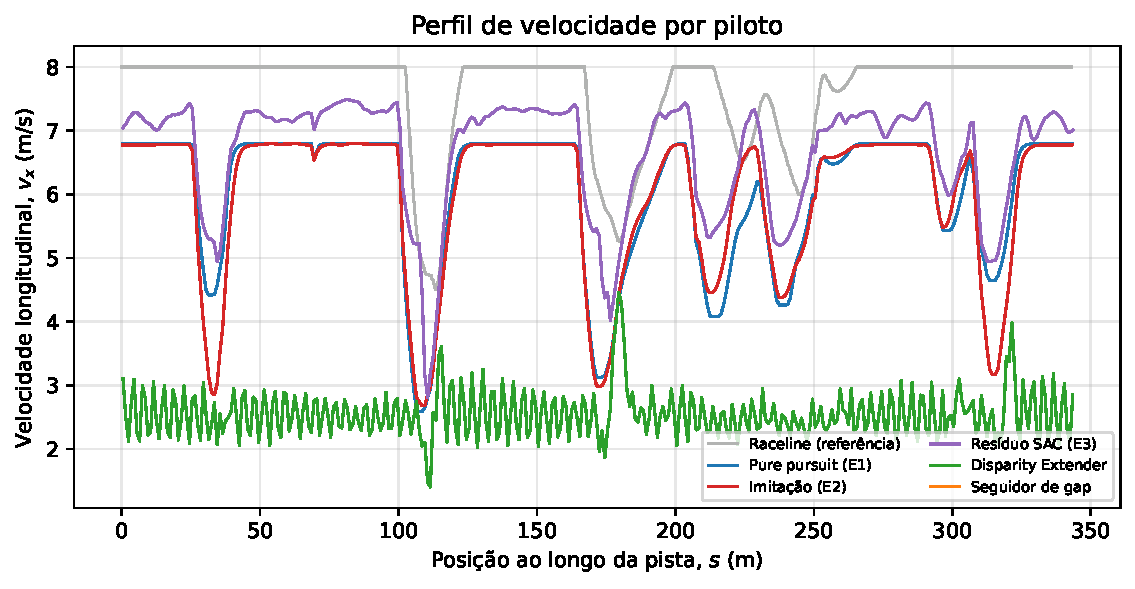
\includegraphics[width=\textwidth]{figs/comparativo/perfil_velocidade}
    \caption{Perfil de velocidade dos pilotos automáticos em Spielberg:
    velocidade longitudinal média por faixa de 1~m da posição $s$ ao longo da
    volta, sobre as voltas completas. A curva cinza é a velocidade de referência
    da linha de corrida}
    \label{fig:cmp_perfil}
\end{figure}

A Figura~\ref{fig:cmp_esterco} põe cada volta completa num plano de taxa de
esterço contra tempo de volta. Os pilotos formam grupos separados, sem
sobreposição entre eles exceto a do E1 com o E2. Não há relação monotônica entre
as duas grandezas: o piloto mais rápido, o E3, esterça mais que o E1 e o E2, e o
mais lento, o Disparity Extender, é também o que mais esterça.

\begin{figure}[htb]
    \centering
    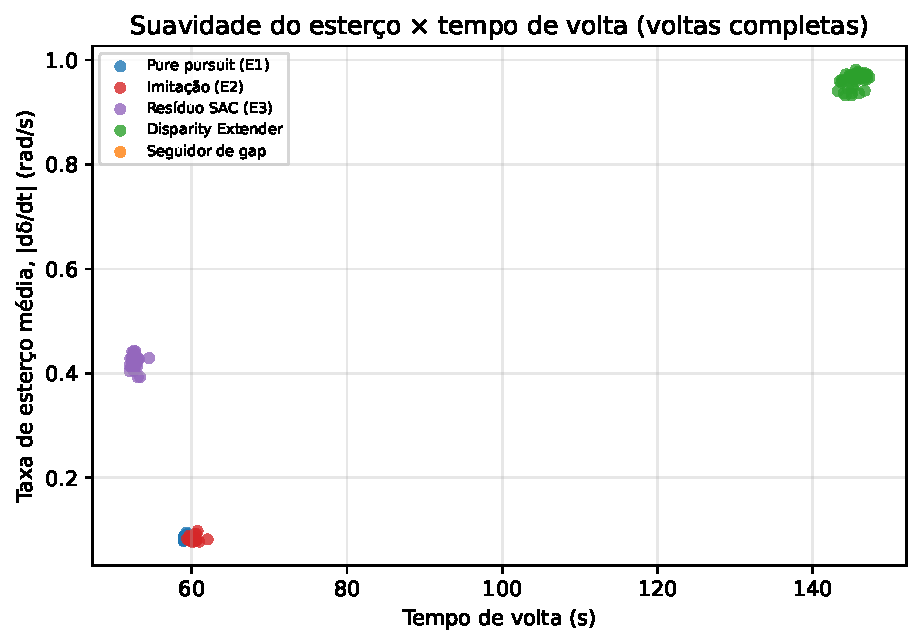
\includegraphics[width=0.85\textwidth]{figs/comparativo/esterco_vs_tempo}
    \caption{Taxa média de esterço contra tempo de volta, uma marca por volta
    completa de cada piloto automático}
    \label{fig:cmp_esterco}
\end{figure}

A Figura~\ref{fig:cmp_trajetorias} mostra, no trecho de maior curvatura da linha
de corrida, a trajetória da volta de tempo mediano de cada piloto. As
trajetórias do E1, do E2 e do E3 praticamente se sobrepõem e acompanham a linha
de corrida de perto. A do Disparity Extender ondula de um lado a outro do
corredor, inclusive na reta de saída, o que é a forma geométrica da sua taxa de
esterço e do seu desvio.

\begin{figure}[htb]
    \centering
    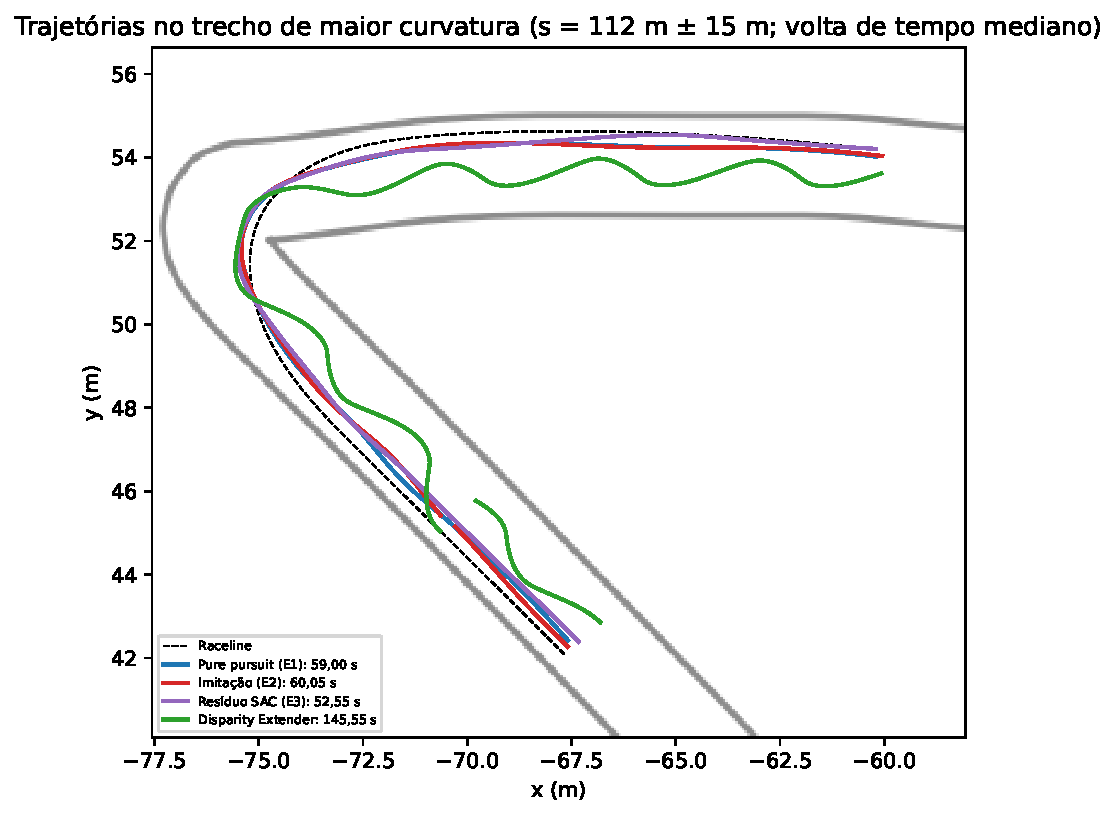
\includegraphics[width=0.85\textwidth]{figs/comparativo/trajetorias_curva}
    \caption{Trajetórias da volta de tempo mediano de cada piloto automático no
    trecho de maior curvatura da linha de corrida de Spielberg, com 15~m para
    cada lado do ponto de maior curvatura. A linha tracejada é a linha de
    corrida. A trajetória do Disparity Extender aparece em dois trechos porque a
    largada sorteada daquela volta caiu dentro da janela: o início e o fim da
    volta passam pelo trecho em momentos diferentes e não se ligam}
    \label{fig:cmp_trajetorias}
\end{figure}

\subsection{Pilotos humanos}\label{sec:res-cmp-humanos}

As sessões humanas seguem o protocolo da Seção~\ref{sec:val-humano}: em cada
vista, dez minutos de treino e três sessões de cinco voltas nas sementes 1000,
1001 e 1002, primeiro com a pista inteira e depois só com o LiDAR. As linhas
humanas da Tabela~\ref{tab:comparativo} estão reservadas e ainda vazias.
Participaram \pendentehumano{número de autores e de voluntários, por grupo e
experiência em jogos de corrida; sessões excluídas e motivo}.

\textbf{Resultado por piloto e vista.} Na vista da pista inteira, os pilotos
humanos completaram \pendentehumano{voltas completas/tentadas, colisões, mediana
e melhor volta, por piloto, autores separados dos voluntários}. Na vista só
LiDAR, \pendentehumano{os mesmos campos na vista só LiDAR}.

\textbf{Tempo real.} O passo de controle humano é segurado até 0,05~s de relógio
e o atraso de cada passo é registrado. Nas sessões que contam,
\pendentehumano{atraso médio, percentil 99 e passos fora do prazo, por sessão}.

A Figura~\ref{fig:cmp_curva} mostra o tempo de cada volta humana na ordem em que
foi feita, do treino às três sessões de cada vista.
\pendentehumano{leitura da curva de aprendizado: tendência no treino, diferença
entre a primeira e a terceira sessão e mudança na troca de vista}.

\begin{figure}[htb]
    \centering
    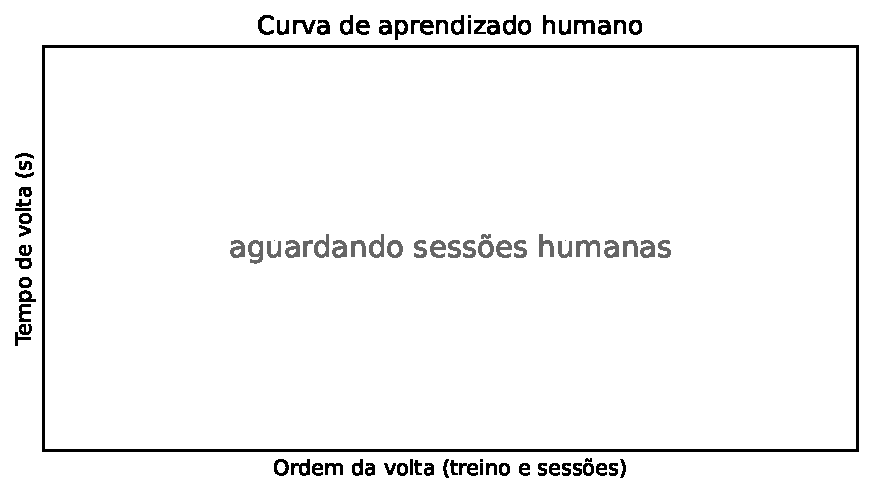
\includegraphics[width=0.85\textwidth]{figs/comparativo/curva_aprendizado}
    \caption{Curva de aprendizado dos pilotos humanos: tempo de volta na ordem
    cronológica, no treino e nas três sessões de cada vista}
    \label{fig:cmp_curva}
\end{figure}

\textbf{Faixa do grupo e posição das políticas.} Por vista, a faixa do grupo
humano --- melhor, mediana e pior piloto pela mediana de tempo de volta --- é
\pendentehumano{faixa do grupo na vista da pista inteira e na vista só LiDAR, e
posição de E1, E2, E3 e Disparity Extender em relação a ela}.

\textbf{Comparação entre as vistas.} Com a mesma pessoa nas duas vistas,
\pendentehumano{diferença de conclusão e de tempo de volta entre a pista inteira
e só o LiDAR, por piloto}. Como a ordem das vistas é fixa, essa diferença mistura
o efeito da informação com o da prática acumulada.

\section{Discussão}\label{sec:res-discussao}

\subsection{O que os números sustentam}

A Tabela~\ref{tab:res_sintese} reúne as etapas da cascata e os demais pilotos
do comparativo na comparação que organiza o argumento do trabalho: desempenho
contra dependência de infraestrutura de percepção. As colunas oficiais são as
dos portões; as do comparativo, as da Seção~\ref{sec:res-comparativo}.

\begin{table}[htb]
    \centering
    \footnotesize
    \setlength{\tabcolsep}{2.5pt}
    \begin{tabular}{|l|c|c|c|c|c|c|c|}
        \hline
        & & \multicolumn{3}{c|}{\textbf{Portão oficial}} &
        \multicolumn{2}{c|}{\textbf{Comparativo}} & \\
        \cline{3-7}
        \textbf{Piloto} & \textbf{Tipo} & \textbf{Volta (s)} &
        \textbf{Razão a $T_{pp}$} & \textbf{Concl.} & \textbf{Volta (s)} &
        \textbf{Concl.} & \textbf{Pose global?} \\
        \hline
        E1 (\textit{pure pursuit}) & clássico & 59,000 & 1,000 & 50/50 & 59,00 &
        44/45 & sim \\
        \hline
        E2 (TinyLidarNet) & ML & 60,050 & 1,018 & 50/50 & 60,05 & 50/50 & não \\
        \hline
        E3 (E2 + resíduo SAC) & ML & 52,525 & 0,890 & 91/92 & 52,55 & 50/50 & não \\
        \hline
        Disparity Extender & clássico & --- & --- & --- & 145,55 & 50/50 & não \\
        \hline
        Seguidor de gap & clássico & --- & --- & --- & --- & 0/5 & não \\
        \hline
        Humano, pista inteira & humano &
        \multicolumn{5}{c|}{\pendentehumano{faixa do grupo}} & vê o mapa \\
        \hline
        Humano, só LiDAR & humano &
        \multicolumn{5}{c|}{\pendentehumano{faixa do grupo}} & não \\
        \hline
    \end{tabular}
    \caption{Síntese dos pilotos em Spielberg. As colunas oficiais são as dos
    portões: o E1 sem randomização, o E2 e o E3 com ela. As colunas do
    comparativo são todas com randomização, cinco sementes de dez voltas;
    a volta é a mediana sobre as voltas completas. Nas linhas humanas, a faixa é
    a do grupo (melhor, mediana e pior piloto)}
    \label{tab:res_sintese}
\end{table}

A cascata faz o que se propôs a fazer. A destilação transfere a competência do
especialista para uma política que enxerga apenas LiDAR e proprioceptiva, ao
custo medido de 1,8\% de tempo de volta; o resíduo recupera esse custo e
\textbf{ultrapassa a política ensinante em 11,0\%}, sem devolver a dependência de
localização, e mantendo a taxa de conclusão acima de 0,98 e a degradação sob
randomização de atrito em zero. Fora do circuito de coleta, a rede destilada
supera o especialista de forma mais dramática ainda, completando voltas em duas
pistas onde o professor completa 16,7\% e 0\%.

Uma assimetria de protocolo favorece a leitura conservadora e vale declará-la. O
denominador $T_{pp}$ é medido \textbf{sem} randomização, enquanto os numeradores
das etapas E2 e E3 são medidos \textbf{com} randomização de atrito, de posição de
largada e de ruído de sensor. A vantagem de 11,0\% do resíduo é, portanto, obtida
por uma política avaliada em condições mais duras que a referência que ela supera.
O braço sem randomização da comparação pareada da etapa E3 permite estimar o
tamanho desse efeito: 52,500~s contra 52,600~s, isto é, cerca de um décimo de
segundo. A assimetria existe, é declarada, e é pequena --- mas ela existe, e um
leitor que compare 52,525~s com 59,000~s deve saber que os dois números não foram
medidos sob o mesmo protocolo.

O comparativo permite fazer essa comparação sob o mesmo protocolo, sem trocar o
número oficial. Com randomização, nas mesmas cinco sementes, o especialista
mediu 59,00~s e o resíduo 52,55~s: a ordem e a distância entre os dois se mantêm,
e a mediana do especialista não se moveu com a randomização. O que a
randomização acrescentou ao especialista foi uma colisão em 45 voltas, e não
tempo de volta.

\subsection{Primeira ressalva: o limiar cai dentro do intervalo de confiança}\label{sec:res-ic}

Nos três portões aprovados, o intervalo de Wilson reportado ao lado da taxa de
conclusão \textbf{contém o limiar}. A Tabela~\ref{tab:val_ic} registra os três
casos, e a Seção~\ref{sec:val-limitacoes} discute a decisão pré-registrada que
leva a isso e quantifica por que o limite inferior do intervalo não pôde ser o
critério nesta escala de amostra. Não se repete aqui essa justificativa; o que
cabe é medir o seu efeito sobre os resultados que este capítulo acabou de
reportar.

O efeito é este: \textbf{se o critério fosse o limite inferior do intervalo, as
três etapas reprovariam} --- a etapa E1 com 0,9287 contra limiar 1,00, a etapa E2
com 0,9287 contra 0,95 e a etapa E3 com 0,9410 contra 0,98. Nenhum dos três
resultados sobreviveria, inclusive os dois que não cometeram uma única falha em
50 voltas. A ressalva não é, portanto, uma sombra sobre um dos portões: ela é
constitutiva de todos eles, e a única forma de removê-la seria medir mais voltas
por configuração avaliada, não escrever o critério de outro jeito.

Convém delimitar o que ela alcança, com os artefatos deste capítulo. Ela alcança
o critério de taxa de conclusão e nenhum outro: os dois critérios de robustez a
atrito da etapa E3 estão a mais de uma ordem de grandeza dos seus limiares, e os
intervalos BCa de tempo de volta ficam inteiramente abaixo dos limiares em E2 e
E3.

O que ela \textit{não} respeita é a fronteira entre aprovar e reprovar, e seria
cômodo supor o contrário --- que uma reprovação, por ser negativa, esteja a salvo
da ressalva que atinge a aprovação. Os artefatos dizem o oposto. Dos quatro
pontos medidos do E3, \textbf{três têm o limiar de 0,98 dentro do intervalo de
Wilson}: os dois que passam no critério de taxa de conclusão e um dos dois que
reprovam nele, como a Seção~\ref{sec:res-e3} abre. Só a reprovação do ponto de 300 mil passos sem
penalidade de proximidade é robusta à escolha de critério, e é a única. Nos
outros três, inclusive na aprovação que é o resultado final do trabalho, a
decisão repousa inteiramente sobre o valor pontual.

Não há como transformar isso numa boa notícia, e a conduta que a
Seção~\ref{sec:val-limitacoes} adota permanece a única defensável. É também a
razão de este capítulo imprimir os quatro intervalos do E3 em vez de só as
quatro taxas: sem eles, o fato de a configuração aprovada e a anterior não se
separarem por intervalo não apareceria em lugar nenhum do trabalho.

\subsection{Segunda ressalva: a realização não é a distribuição}

A segunda ressalva é mais severa que a primeira e atinge especificamente a etapa
E3. A Tabela~\ref{tab:val_sensibilidade} mede a sensibilidade das duas políticas
a perturbação numérica irrelevante, e a Seção~\ref{sec:val-limitacoes} analisa o
que ela implica: a amplitude é de \textbf{0,0381} para a política composta e
\textbf{nula} para a rede de imitação isolada.

O que este capítulo acrescenta é a confrontação dessa amplitude com as margens
que ele acabou de reportar. A margem da etapa E3 sobre o seu limiar é
$0{,}9891 - 0{,}98 = 0{,}0091$; a amplitude sob perturbação irrelevante é
0,0381, \textbf{mais de quatro vezes maior}. A margem da etapa E2 sobre o seu
limiar é 0,05, contra amplitude nula. Em outras palavras: a aprovação da etapa E2
é robusta à realização numérica da política, e a da etapa E3 não é.

A consequência precisa ser dita sem atenuação. \textbf{Para a etapa E3, o número
reproduzível é a distribuição, não a realização.} Quem reimplementar a
composição com outra ordem de operações, outro tipo de ponto flutuante ou outra
versão da biblioteca de álgebra medirá outro valor dessa faixa, e esse valor
pode ficar abaixo do limiar. O 0,9891 da Tabela~\ref{tab:res_e3_criterios} é uma
realização legítima, medida com a composição única que o contrato numérico
determina, num artefato com proveniência íntegra --- e não é um valor que se deva
esperar reproduzir dígito a dígito noutra implementação.

Duas qualificações fecham o ponto. A primeira é de escopo, e coincide com a da
ressalva anterior por um motivo diferente: como a perturbação reembaralha
\textit{qual} episódio termina em colisão sem deslocar o resultado numa direção,
ela atinge a contagem de voltas e não o tempo de volta, cuja mediana no E3 tem
intervalo BCa de apenas 0,21~s de largura. A segunda é mais incômoda: o estudo de
sensibilidade foi feito na máquina anterior do projeto, cujas execuções não
sobreviveram à migração --- fato declarado na Seção~\ref{sec:val-limitacoes}. A
confrontação entre margem e amplitude que esta subseção faz combina, portanto, um
número auditável nesta máquina com uma amplitude medida numa execução que já não
é reconferível. Reproduzir o estudo neste host é a forma de fechar a lacuna, e
não foi feito.

\subsection{Terceira ressalva: a sobreposição do conjunto de generalização}

A sobreposição entre o conjunto de coleta e o conjunto de generalização foi
tratada duas vezes: a Seção~\ref{sec:val-heldout} expõe o defeito de desenho que
a produz, mostra por que ele era mais grave para execuções futuras do que para a
execução reportada, explica por que a correção não pôde ser aplicada
retroativamente e registra a regra que a fechou para as execuções seguintes; a Seção~\ref{sec:res-e2} deste capítulo acrescenta a metade
recíproca, que a mesma coleta foi causalmente necessária.

O que resta dizer, e é a consequência prática para quem lê os números, cabe em
duas linhas. \textbf{Nenhum valor deste capítulo deve ser citado como
``generalização em três pistas não vistas''}: das três pistas que pontuam o
critério, apenas Oschersleben é inteiramente inédita. E o valor de generalização
do E3 simplesmente não existe --- o resíduo nunca foi avaliado fora de
Spielberg, o que é o segundo item da lista da subseção seguinte, e não uma
variante desta ressalva.

\subsection{O que os números não sustentam}

Além das três ressalvas acima, seis limites delimitam o alcance dos resultados
deste capítulo. Nenhum deles é atenuado.

\begin{itemize}
    \item \textbf{Uma execução por configuração.} Os quatro pontos da
          Tabela~\ref{tab:res_e3_pontos} diferem por uma variável cada, mas cada
          ponto é \textit{um} treino. A variabilidade entre sementes de
          \textbf{treino} não foi medida em nenhuma etapa --- as 5 ou 10
          sementes dos portões são de \textbf{avaliação}, sobre um ponto de
          verificação fixo. A diferença entre as duas últimas configurações ---
          três colisões contra uma --- é atribuída à penalidade de proximidade
          porque foi a única variável alterada, mas o trabalho não mediu quanto
          dessa diferença caberia dentro da dispersão de dois treinos com a
          mesma configuração e sementes distintas. Essa é a lacuna mais direta a
          fechar.
    \item \textbf{Um circuito de portão.} Todos os critérios de aceite das três
          etapas são medidos em Spielberg. As outras quatro pistas entram apenas
          no critério de generalização da etapa E2, e nenhuma delas pontua a
          etapa E3: o resíduo não foi avaliado fora do circuito em que treinou.
    \item \textbf{Um simulador e um modelo de veículo.} A fidelidade do modelo
          de faixa única é premissa herdada, e a Seção~\ref{sec:val-colisao}
          registra que o detector de colisão do simulador precisou ser corrigido
          antes que qualquer número deste capítulo fosse reportável --- o que é
          evidência a favor da desconfiança, não contra ela.
    \item \textbf{Veículo único, sem corrida direta.} Não há ultrapassagem, nem
          oponente, nem obstáculo dinâmico, pelos motivos que a
          Seção~\ref{sec:arte-lacuna} declara.
    \item \textbf{Nenhum resultado fora da simulação.} Toda comparação
          numérica deste capítulo com resultados de campo da literatura é
          assimétrica, e assim deve ser lida.
    \item \textbf{A evidência não é durável.} Os relatórios que sustentam cada
          número deste capítulo não são versionados, e o relatório de
          verificação é sobrescrito a cada execução, de modo que medições
          feitas por esse relatório não podem ser reconferidas depois. No
          comparativo, o resumo das execuções --- tabela, figuras, dados
          agregados e registros das varreduras --- está versionado junto com
          este texto, mas os dados passo a passo, não.
\end{itemize}

\subsection{O comparativo: controladores clássicos e de aprendizado de máquina}\label{sec:res-disc-cmp}

\textbf{Mesma informação, desempenhos distintos.} Quatro pilotos do comparativo
executam apenas com LiDAR e proprioceptiva: o E2, o E3 e os dois reativos. Sob o
mesmo protocolo, os dois aprendidos completam 50 de 50 voltas em 60,05~s e
52,55~s; o Disparity Extender completa 50 de 50 em 145,55~s; e o seguidor de gap
não completa volta. O único piloto que usa pose global e linha de corrida, o
E1, fica em 59,00~s. Com o mesmo sensor em execução, as políticas aprendidas
chegaram ao tempo do piloto que usa o mapa, e uma delas o superou; os
controladores reativos, não.

\textbf{O que essa comparação não diz.} Ela compara estas implementações, e não
as famílias de método. Três diferenças entre os dois lados precisam acompanhar
os números. Os reativos são portes de nós escritos para um veículo real lento,
ajustados por uma varredura de no máximo 24 combinações por grade (48 no
seguidor de gap, que teve duas grades), e a configuração do
Disparity Extender ficou no limite da sua grade. Os aprendidos passaram por laços
automáticos com várias tentativas e ações pré-declaradas (Seções~\ref{sec:res-e2}
e~\ref{sec:res-e3}). E, sobretudo, os aprendidos foram treinados com
demonstrações de um especialista que usa pose e linha de corrida: eles não
precisam do mapa em execução, mas a informação do mapa de Spielberg entrou neles
pelo treino. Os reativos não têm acesso a essa informação em momento algum. A
vantagem que eles teriam --- funcionar num circuito desconhecido, sem mapa e sem
treino, como argumenta a Seção~\ref{sec:arte-classico} --- não é medida aqui,
porque o comparativo usa uma só pista.

\textbf{Suavidade e desvio.} O E1 e o E2 têm a mesma taxa de esterço,
0,08~rad/s; o E3, o mais rápido, sobe para 0,42~rad/s;
o Disparity Extender tem a maior taxa, 0,97~rad/s, e o maior tempo. A taxa de
esterço, sozinha, não ordena os pilotos por desempenho, e a
Figura~\ref{fig:cmp_esterco} mostra que não há relação monotônica entre as duas
grandezas. O desvio da linha de corrida também não é medida de qualidade: o E3
se afasta mais dela que o E1 e o E2 (0,40~m em média, contra 0,26 e 0,27~m) e é o
mais rápido. O que o desvio mede é a semelhança com o especialista, cuja
referência é a própria linha de corrida.

\textbf{Por que o seguidor de gap não completa volta.} Os dados das varreduras
são compatíveis com dois mecanismos, que se somam. O primeiro está na escolha do
alvo. A detecção por descontinuidade define uma abertura por um salto de alcance
maior que o limiar de profundidade entre pontos consecutivos do \textit{scan}.
Numa pista fechada e sem obstáculos, as paredes produzem um \textit{scan}
contínuo, exceto onde uma parede próxima esconde um trecho mais distante, o que
ocorre tipicamente na borda interna de uma curva. As bordas das aberturas
candidatas caem, assim, sobre a própria parede, e o alvo, pontuado por distância e
largura, fica junto a uma dessas bordas, e não no centro do corredor livre. O
Disparity Extender, ao contrário, estende cada disparidade pela largura do carro
antes de escolher, o que afasta o alvo da borda. O segundo mecanismo é a
oscilação do esterço. Com ganho proporcional de 1,5 ou 2,2, a taxa média de
esterço por combinação da grade oficial ficou entre 0,41 e 1,98~rad/s, contra
0,08~rad/s do E1, o que é compatível com um esterço que oscila entre os limites:
com o atraso de dois passos (100~ms), o PID corrige um erro que o carro já deixou
para trás, e um ganho alto transforma essa defasagem em oscilação. A isso se soma
a saturação: o nó original permitia 0,7~rad de esterço, e o porte corta em
0,4189~rad, como todos os pilotos.

A grade ampliada separa os dois mecanismos, e é por isso que ela é informativa
apesar de não ter produzido volta. Com ganho de 0,3, a taxa média de esterço,
medida como média do episódio de sonda, caiu para 0,08 a 0,29~rad/s, e, com a
velocidade comandada pelo PID, para 0,08 a 0,11~rad/s, perto dos 0,08~rad/s do E1
e do E2 (na tabela, essa grandeza é a mediana, entre voltas completas, da média
de cada volta, de modo que a comparação é de ordem de grandeza), e o carro
continuou batendo
nos primeiros metros, com progresso médio de no máximo 8,20~m. Um esterço suave
não bastou, o que aponta a escolha do alvo como causa dominante --- e a escolha do
alvo não depende de nenhum dos parâmetros varridos. Esta é uma interpretação de
dados agregados: o alvo escolhido a cada passo não foi gravado, e confirmá-la
exigiria gravá-lo. O que não depende de interpretação é o resultado, obtido pelo
critério fixado antes da medição: o seguidor de gap, nesta implementação e neste
regime de velocidade e atraso, não completa uma volta em Spielberg.

\textbf{A comparação com os pilotos humanos.} O desenho é descritivo e não tem
teste de hipótese (Seção~\ref{sec:val-humano}). O que ele permite dizer é a
posição de cada política em relação à faixa do grupo humano, vista a vista, e a
leitura de cada vista foi fixada antes da coleta. Na vista só LiDAR, humanos e
políticas sem pose recebem informação equivalente --- o \textit{scan} atual,
dentro de um alcance fixo, e a velocidade no painel ---, e a diferença entre eles é de
decisão e de controle; na vista da pista inteira, o humano vê o mapa e pode
antecipar as curvas, e a diferença mistura habilidade com informação. Com os
dados, \pendentehumano{posição de E1, E2, E3 e Disparity Extender em relação à
faixa do grupo, por vista}.

Dois cruzamentos têm leitura direta. O primeiro é entre o humano na vista só
LiDAR e o seguidor de gap, que reagem ao mesmo \textit{scan} do passo atual:
\pendentehumano{se e quanto os humanos na vista só LiDAR completaram as voltas que
o seguidor de gap não completa}. O segundo é a suavidade:
\pendentehumano{taxa de esterço e desvio da linha de corrida dos humanos diante
das políticas}. Das limitações da Seção~\ref{sec:val-limitacoes-comparativo},
cinco acompanham qualquer uma dessas leituras: a informação desigual na vista da
pista inteira, a ordem fixa das vistas, a amostra pequena, a separação entre
autores e voluntários e a pista única.


\subsection{Síntese}

O resultado quantitativo do trabalho é uma política que enxerga apenas LiDAR e
proprioceptiva, completa 91 de 92 voltas sob randomização de atrito, posição de
largada e ruído de sensor, e percorre o circuito em 52,525~s --- 11,0\% mais
rápido que o especialista geométrico que originou os seus rótulos e que depende
de pose global para funcionar. A cascata de três etapas preserva, em cada passo,
a propriedade conquistada no anterior: o especialista fornece competência, a
imitação a transfere para uma política sem pose global, e o resíduo recupera e supera
o desempenho perdido na destilação sem devolver a dependência de localização, com
o pior caso da terceira etapa sendo o resultado da segunda.

Sob o protocolo comum do comparativo, a ordem se mantém: com randomização e nas
mesmas cinco sementes, o resíduo faz 52,55~s, o especialista 59,00~s e a rede de
imitação 60,05~s. Dos dois controladores reativos que usam apenas o LiDAR, o
Disparity Extender completa todas as voltas em 145,55~s, e o seguidor de gap não
completa nenhuma, nem nas 48 combinações das duas varreduras nem na avaliação
congelada. Quanto aos pilotos humanos, \pendentehumano{uma frase com a posição das
políticas diante da faixa do grupo humano em cada vista}.

O resultado metodológico é de outra natureza e, no julgamento deste trabalho, é o
mais transferível dos dois. As três ressalvas discutidas acima --- o limiar dentro
do intervalo, a sensibilidade da política composta a perturbação irrelevante, e a
sobreposição entre o conjunto de generalização e as ações de correção --- não
foram descobertas por um revisor depois do resultado. Duas delas estavam
declaradas, com o motivo quantificado, \textbf{antes} de qualquer medição, e a
terceira foi encontrada conferindo o artefato contra o texto que o descrevia, e
declarada em vez de corrigida retroativamente, porque corrigi-la depois de ver o
número seria o defeito maior. Um capítulo de resultados que apresentasse apenas os
valores da Tabela~\ref{tab:res_sintese} teria omitido o que este trabalho de fato
tem de incomum: não os números, mas a possibilidade de dizer com precisão o que
eles não sustentam.
